\documentclass[runningheads]{llncs}
\usepackage[english, USenglish, american]{babel}
\usepackage{ucs}
\usepackage{forest} % for diagrams
\usepackage{tikz-qtree} % for digramas
\usepackage{framed}
\usepackage[utf8x]{inputenc} 							% Encoding (allows accents)
\usepackage[printonlyused,nolist]{acronym}	% Acronyms (print only used)
\usepackage{cite}% Allow multiple citations, etc.
\usepackage{indentfirst} 								% Allow indent on first paragraph
% \usepackage[pdftex]{graphicx}
\usepackage{graphicx} 									% Pictures
\usepackage[cmex10]{amsmath}
\usepackage{amssymb}
\usepackage{mathtools}									% Maths
\usepackage{algorithmic}
\usepackage{algorithm}
\usepackage{array}
\usepackage{mdwmath}
\usepackage{tabularx} %useful in equations
\usepackage{mdwtab}
\usepackage{eqparbox}
\usepackage{longtable}
\usepackage{lscape}
\usepackage{rotating}
\usepackage[raggedright]{sidecap} % for side captions
\usepackage{multirow}
\usepackage{hyphenat}
\usepackage[export]{adjustbox}
\usepackage{alltt}
\usepackage{booktabs}
\usepackage[tight,footnotesize]{subfigure}
\usepackage[hyphens]{url}
\usepackage{pdflscape}									% Allow horizontal pages (in the pdf too)
\usepackage[breaklinks=true]{hyperref}
\usepackage{color}
\usepackage[left]{lineno}
\usepackage[textwidth=2.8cm,disable]{todonotes}
\setcounter{tocdepth}{3}
\hyphenation{op-tical net-works semi-conduc-tor}
\setlength{\parindent}{0.5cm}
\setcounter{secnumdepth}{3}
\selectlanguage{USenglish}

\newcommand{\keywords}[1]{\par\addvspace\baselineskip\noindent \textbf{Keywords:} \enspace\ignorespaces#1}

\usepackage{caption} 
\usepackage{enumitem}
\captionsetup[table]{skip=5pt}
\usepackage{listings} 									% Source code blocks
\usepackage[toc,page]{appendix}							% Appendix
\usepackage{qtree}
\usepackage{wrapfig}
\usepackage{newfloat}
\renewcommand{\arraystretch}{1.2} % increase space in tables
\setlength{\tabcolsep}{.25em} % increase horizontal space in tables


%reduce space between the figure and remaining text
\setlength{\textfloatsep}{1\baselineskip plus 0.2\baselineskip minus 0.5\baselineskip}


\usepackage{amssymb}% http://ctan.org/pkg/amssymb
\usepackage{pifont}% http://ctan.org/pkg/pifont
\newcommand{\cmark}{\ding{51}}%
\newcommand{\xmark}{\ding{55}}%


\usepackage{xparse}% http://ctan.org/pkg/xparse
% Rotation: \rot[<angle>][<width>]{<stuff>}
\NewDocumentCommand{\rot}{O{45} O{1em} m}{\makebox[#2][l]{\rotatebox{#1}{#3}}}%



\begin{document}

%%%%%%%%%%%%%%%%%%%%%%%%%%%%%%%%%%%%%%%%%%%%%%%%%
% For REVIEW
% \linenumbers
%%%%%%%%%%%%%%%%%%%%%%%%%%%%%%%%%%%%%%%%%%%%%%%%%

%%%%%%%%%%%%%%%%%%%%%%%%%%%%%%%%%%%%%%%%%%%%%%%%%
% fix TOC on llncs
%%%%%%%%%%%%%%%%%%%%%%%%%%%%%%%%%%%%%%%%%%%%%%%%%
\makeatletter 
\renewcommand*\l@author[2]{}
\renewcommand*\l@title[2]{}
\makeatletter
%%%%%%%%%%%%%%%%%%%%%%%%%%%%%%%%%%%%%%%%%%%%%%%%%

\mainmatter
\title{Rapport - Establishing Harmonious Relationship Between Robots and Humans}
\titlerunning{Rapport}
\authorrunning{Rapport}

\author{Bruno Alexandre Pires Henriques\\
	\email{bruno.p.henriques@tecnico.ulisboa.pt}
}
\authorrunning{Bruno Henriques}
\institute{
	Prof. Ana Paiva\\
	Prof. Rui Prada\\
	Universidade de Lisboa\\
	Técnico Lisboa (Taguspark)\\
	Av. Prof. Dr. Aníbal Cavaco Silva\\ Porto Salvo, Portugal\\
	\url{http://www.tecnico.ulisboa.pt}\\
}

\maketitle

%%%%%%%%%%%%%%%%%%%%%%%%%%%%%%%%%%%%%%%%%%%%%%%%%%%%%%%%%%%%%%%%%%%%%%%%%%%%%%%%%%%%%%%%%%%%%%%%%%%%%%%%%%%%%%%%%%
% ABSTRACT
\begin{abstract}

Autonomous agents are becoming our next companions. They may be able to offer physical therapy assistance, play games and even help us treat weight loss. However, it is not enough to build agents that are socially engaging and attractive at first, they need to continuously convey such feelings and encourage user interactions, i.e., to build and maintain rapport over long periods of time. In this work, we propose a novel approach for learning subconscious behaviours from humans based on limited-perception \acl{WoZ} with human experts to provide corrective feedback in order to create a generic ``rapport'' model for an autonomous agent. The proposed method will be incorporated, trained, and tested on a robotic rapport agent, \acs{EMYS}, set up in a negotiation scenario, the Split Or Steal game. Following current literature on rapport and \acs{HRI}, we propose a hybrid architecture that combines both rule-based and \acl{ML} based components. On the first component we model high-level behavioural rules that are easier to specify, and on the second component, we use \acl{RL} techniques to generate correct backchannels (listener behaviours) that would be harder to specify otherwise. Lastly, we will evaluate the effectiveness of the proposed approach on learning subconscious behaviour, the quality of the rapport agent, and the impact of rapport on cooperation in the negotiation scenario.

\keywords{Rapport, Backchannel, \acl{RL}, \acl{ML}, \acl{HRI}, \acs{SERA}, \acl{WoZ}, \acs{EMYS}}
\end{abstract}
%%%%%%%%%%%%%%%%%%%%%%%%%%%%%%%%%%%%%%%%%%%%%%%%%%%%%%%%%%%%%%%%%%%%%%%%%%%%%%%%%%%%%%%%%%%%%%%%%%%%%%%%%%%%%%%%%%


%%%%%%%%%%%%%%%%%%%%%%%%%%%%%%%%%%%%%%%%%%%%%%%%%
% Table of content
\newpage
\tableofcontents
\newpage
%%%%%%%%%%%%%%%%%%%%%%%%%%%%%%%%%%%%%%%%%%%%%%%%%

%Humor -> Treger2013
%(e.g. facial expression mirroring \cite{Dimberg2000, Hess1999})
%%%%Baxter2014%%%%%%%%%%%%%%%%%%%%%%%%%%
%objective characterisation of the gaze behaviour of the human towards the robot during an interaction, and explore how this analysis can shape the assessment of the human’s behaviour, and the state of the interaction itself.

%human gaze behaviour over the course of an interaction can provide useful information regarding the state of the interaction, and also the attitude of the human towards the robot.
%%%%%%%%%%%%%%%%%%%%%%%%%%%%%%%%%%%%%%%

%Moreover, the personality of the listener's can impact negatively the results because, as described, after several iterations the model converge to the average speaker and listener \cite{Kok2012}.

% assess... denote... usefulness... applicability of the the prposed methodonlogy, bears, beforehand, thus..., In that respect, ... accusttomed... as illustrated in FIg X., As discussed in Sec. ... endeavor


%NORMALIZAR TUDO PARA limited-perception WoZ


\section{Introduction}
\label{sec:Introduction}
Robots are increasingly becoming part of our society and their presence has been proven to impact our lives. But do any of us remember a remarkable interaction with a robot to the same degree we are able to recall one with a person? What makes one conversation memorable? People can do this so easily and establish rapport rapidly. How can we design robots that can achieve something that has so much impact?

In order to answer these questions, the \ac{HRI} research community has been exploring agents capable of responding emotionally and more humanly in dyadic interactions. More specifically, researchers have been exploring how to exhibit signs of friendliness, coordination, and attentiveness in dyadic interactions. In other words, researchers have been studying how to develop rapport agents. These agents are being applied in several domains such as education~\cite{Burroughs2007}, autism~\cite{Feil-Seifer2009, Scassellati2012}, child care~\cite{Burns1984}, medical assistances~\cite{Kang2005, Lisetti2013}, family companions~\cite{Bickmore2005}, weight loss~\cite{Fasola2012}, and several other examples~\cite{Marti2006, Nadler2003}.

In order to improve the agents' performance, several studies were conducted to identify how to influence people using different verbal and non-verbal strategies. There is evidence in these studies that rapport agents can make people feel: more connected~\cite{Rosenthal-vonderPutten2013, Tsai2012}, less tense~\cite{Wang2010}, less embarrassed~\cite{Kang2009}, and more capable of trusting~\cite{Kang2009}. However, the impact depends on how such strategies are executed. For example, a poorly timed head nod, a backchannel to generate coordination and attentiveness, may reduce rapport.

Despite present efforts regarding rapport, there are still important issues that can be further improved and the proposal intends to address, namely:
\begin{enumerate}[label=(\roman*)]
	\item Lack of studies on how backchannels \ac{ML} based prediction models benefit from \ac{WoZ} studies;
	\item Methods to train virtual agents to simulate subconscious human behaviour;
	\item Lack of robotic rapport agents that is capable of eliciting every component of rapport: positivity, coordination and mutual attention.
\end{enumerate}

We propose extending the \ac{SERA}\cite{Tullio2015} framework to manage rapport in dyadic settings because it is integrated into several robotic agents, and because it is being developed internally in \ac{GAIPS}. The proposed solution will use a hybrid architecture with one rule-based component to model high-level interactional rules that are easy to specify, and two \ac{ML} based components to model appropriate timings and actions for backchannels, respectively. Following current literature, we will use \ac{RL}~\cite{Thomaz2006, Kok2012, Zhao2014, Papangelis2014, Blumberg2002, Andrist2015, Mutlu2006} (Section~\ref{subsec:ReinforcementLearning}).

The \ac{ML}-based components will be trained using a novel approach to learn subconscious human behaviours based on a modified limited perception \ac{WoZ}~\cite{Sequeira2016, Knox2014} with human experts providing corrective feedback.

To evaluate the proposed solution, a rapport agent will be developed, trained and tested on a dyadic negotiation game setting based on the Split Or Steal game using robot \ac{EMYS}. We expect the developed system to stimulate the essential components of rapport: positivity through the rule-based component, and attentiveness and coordination through the previous learnt \ac{ML} models. The evaluation will measure the effectiveness of the proposed approach on learning subconscious behaviour, the quality of the rapport agent, and the impact of rapport on cooperation in the proposed negotiation scenario.

\subsection{Objectives and Expected Contributions}
\label{subsec:Objectives}

The main goal is to improve current predictive models for backchannels (which are essential to build rapport agents) to be used on robots with inherent limitations over the environment, regarding its perceptions and actions. To solve this issue, we propose to:

\begin{enumerate}[label=(\roman*)]
	\item Extend the \ac{SERA} framework to support rapport management using a hybrid controller with a rule-based component, and two \ac{ML}-based components trained with the proposed approach;
	\item Create a rule-based component for managing rapport which will be the baseline for training and evaluation;
	\item Train a \ac{ML} classifier to assess socially adequate timings for backchannel generation;
	\item Train a \ac{ML} classifier to determine the most appropriate backchannel during interactions;
	\item Integrate the rapport agent on a negotiation scenario, Split Or Steal game;
	\item Conduct a study to compare the final rapport agent with the baseline.
\end{enumerate}

Lastly, the expected contributions of this proposal are:
\begin{enumerate}[label=(\roman*)]
	\item A novel approach to learn subconscious information from human subjects based on a limited-perception \ac{WoZ}~\cite{Sequeira2016};
	\item Studies over the impact of our proposed approach over training backchannels predictive models;
	\item Improvement over previous rapport agents regarding their quality and naturalness;
	\item Extension of \ac{SERA} framework to support rapport management in dyadic interactions.
\end{enumerate}

The remainder of the document is organised as follows. Section \ref{sec:Background} describes rapport, \acl{ML}, and \acl{RL}. Section \ref{sec:StateOfTheArt} describes the current state-of-art in rapport agents. Sections \ref{sec:Solution} and \ref{sec:Evaluation}, describe, respectively, the proposed solution and the implementation and methodology for evaluation. Lastly, the conclusions and the planning will be addressed in Section~\ref{sec:Conclusion}.
\section{Background}
\label{sec:Background}

For the following sections, the main concepts of the document will be described. Section~\ref{subsec:Rapport} describes the concept of rapport since it is the main phenomenon we want to elicit on people's perception. Currently, researchers have been starting to use \acl{ML} approaches which Section~\ref{subsec:Rapport} describes. Lastly, Section~\ref{subsec:ReinforcementLearning} describes \acl{RL} \ac{ML} techniques, following current suggestions made by several researchers~\cite{Thomaz2006, Kok2012, Sequeira2016, Zhao2014, Papangelis2014}.

\subsection{Rapport}
\label{subsec:Rapport}
The feeling of flow and connection during interactions is formally known as rapport~\cite{Wang2009}. It is a phenomenon that affects people on three levels: emotional, behavioural and cognitive~\cite{Wang2009}.

The emotional level refers to the impact the relationship has on partners, while behavioural refers to, for example, the convergence of movements and facial expressions. Finally, the cognitive level refers to a shared understanding between conversational partners~\cite{Wang2009}.

Spender Oatey~\cite{Spencer-Oatey2005} suggests that rapport management can be divided into three main tasks: enhancement, maintaining and destroy. The first task aims to create strong first impressions, the second encourages the continuation and the third task aims to destroy relationships. Each one of these tasks can be modelled as abstract goals that can be accomplished by achieving sub-goals only satisfied by interacting with the external world~\cite{Papangelis2014, Zhao2014} (see Figure~\ref{table:BuildingRapportPlan}). These sub-goals manipulate the three components of rapport suggested by Tickle-Degnen and Rosenthal~\cite{Tickle-Degnen1990}:

\begin{itemize}
	\item \textbf{Positivity}: feeling of approval and friendliness (e.g. head nod and smile);
	\item \textbf{Mutual attention}: feeling that the other's attention is focused on the individual (e.g. mutual gaze and ``hmm hmm'' vocalisations);
	\item \textbf{Coordination}: feeling of predictability and being in-sync (e.g. postural mimicry and synchronised movements).
\end{itemize}

\vspace{-5mm}
\begin{figure}
	\centering
	%\begin{framed}
		\scalebox{0.65}{
			\begin{forest}
				[\textbf{Build Rapport}
				[Stimulate Positivity 
					[Elicit Positive emotions [Smile] [Embarrassed Laugh][Praise]]]
				[Stimulate Mutual Attention
					[Mutual Gaze] [Voice utterances][Paraphrasing]]
				[Stimulate Coordination
					[Postural Mirror]
					[Be predictable
						[Adhere To Social Norms
							[Greet] [Be Polite]]]]
				]
			\end{forest}
		}
	%\end{framed}
	\caption{Example plan for building rapport. The nodes are goals and the leafs are actions.}
	\label{table:BuildingRapportPlan}
\end{figure}
\vspace{-4mm}

However, in order to build rapport, it is essential that these three components co-exist during an interaction~\cite{Grahe1999, Wang2010, Zhao2014, Cassell2007}. For example, using gaze to establish mutual attention conveys disinterest and can have negative social effect if not accompanied by other behaviours that stimulate positivity and coordination~\cite{Wang2010}. Although, the relative weights of these components may change as the relationship evolves beyond strangers~\cite{Wang2010, Zhao2014, Cassell2007}.

Moreover, two strangers behaviours are initially driven by cultural conventions as they do not know each other and, therefore, they expect what was taught by their cultural environment according to the current context~\cite{Zhao2014} (e.g. greet and be polite). As the relationship evolves and the interlocutors get to know one another, positivity decreases and it is replaced by coordination while mutual attention remains constant~\cite{Zhao2014, Tickle-Degnen1990}. The interlocutors may even violate what is culturally accepted in order to meet interactional goals and behavioural expectations~\cite{Zhao2014}. For example, friends may use sarcasm and insults instead of politeness~\cite{Zhao2014}. Table~\ref{table:rapportStrategies} describes examples of verbal and non-verbal strategies for managing rapport.

\vspace{-3mm}
\begin{table}[]
	\centering
	\begin{tabular}{@{}ll@{}}
		\toprule
		\multirow{2}{*}{\textbf{Verbal}}    & Humour; Paraphrasing; Self disclosure; Praise; Ego Suspension.\\ 
		& Refer to shared experience; Slower rate of speech; Small-talk; \\ \midrule
		\multirow{2}{*}{\textbf{Non-verbal}} & Gaze; Smile; Reciprocate previous action. Silence; Postural mimicry; \\  
		& Gesture mimicry; Mirror Facial Expression; Head gestures. \\ \bottomrule
	\end{tabular}
	\caption{Examples of strategies and actions to manage rapport.}
	\label{table:rapportStrategies}
\end{table}
\vspace{-8mm}

Learning behavioural expectation is also important to assess rapport success. This can be achieved through the use of self-disclosure \cite{Moon2000}, small-talk~\cite{Cassell2003} and humour~\cite{Treger2013}. For instance, when self-disclosure is successful, it is reciprocal, intimacy increases, disclosed topics become more diversified, and deeper~\cite{Zhao2014}. Moreover, assessing when rapport strategies were successful is also important, for example, mutual gaze and smiling become more noticeable and consistent\cite{Grahe1999, Zhao2014}.

To sum up, rapport is a phenomenon that makes interactions more engaging and harmonious. Rapport management can be modelled as a problem of goal satisfaction that is solved through the realisation of actions. However, the strategies for managing rapport must take into account the goals of the interaction and the sociocultural context of the interaction in order to satisfy behavioural expectations. Although, these expectations may not be clear at first and strategies for learning them should be applied.
\subsection{\acl{ML}}
\label{subsec:MachineLearning}

\acf{ML} is a subfield in Computer Science that develops algorithms capable of automatically learn and make predictions based on data~\cite{Bishop2006}. In supervised learning, the data is retrieved from datasets or corpus, and in unsupervised learning, the data is directly sampled from the interaction. Despite not requiring handcrafted rules, these algorithms requires large amounts of quality data and good discriminative features in order to create good predicting models or classifiers. However, acquiring great amount of data may prove difficult in \ac{HRI} since it takes a great toll on the development design as it requires careful preparation, feature selection, data processing techniques, and most of all, test subjects (Figure~\ref{fig:MLDiagram}).

In addition, preliminary studies, in the intended scenario, are crucial to assess the most relevant interactions, and behavioural features we have to look before starting the training stage (see relation between the dataset and training in Figure~\ref{fig:MLDiagram}). One must take into account that excessive features may lead to redundancy (noise) contributing negatively to the quality of the classifier (overfitting). Therefore, it is recommended to use less features in order to have better generic model.

% REMOVED ADDED IF I HAVE SPACE (HALF PAGE)
%Most \ac{ML}-algorithms use eager learning techniques where the models produce global approximations to the given dataset however, there are another algorithms (e.g., $k$-nearest neighbours) that use lazy learning~\cite{Atkeson1997} to produce local approximations. These algorithms store the training dataset locally that is only used when given a test sample. Depending on the intended scenario, the latter approach may return better results. For example, eager learning may model a graph curve using a liner function (global approximation) whether lazy learning may use several liner functions (local approximations).


\begin{figure}[hbt]
  \centering
  %\begin{framed}
	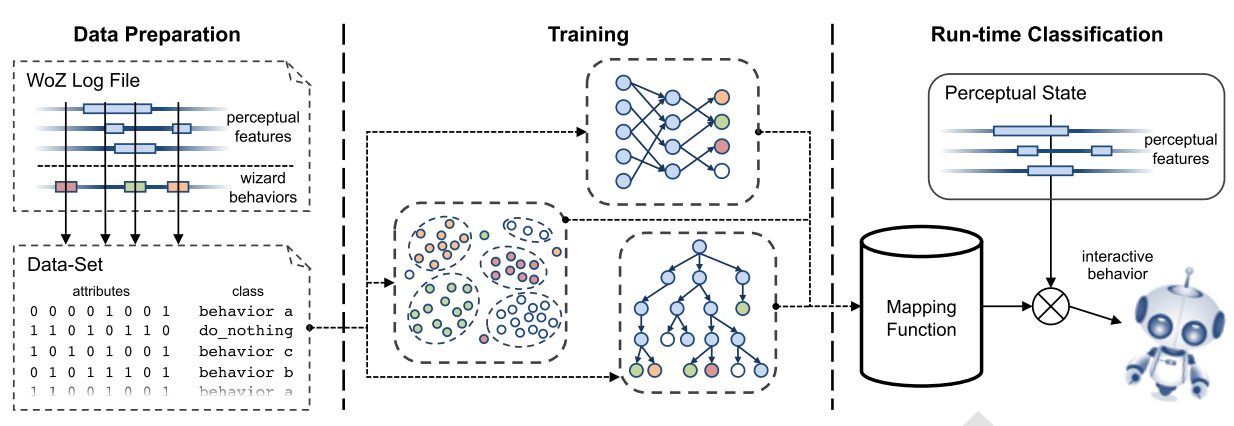
\includegraphics[width=\textwidth]{images/RestrictedPerception_ML_Diagram.png}
  %\end{framed}
  	\caption{Illustration of a \ac{ML} system in a \ac{HRI} application. The dataset is collected and prepared, then it is given to a \ac{ML} algorithm, and lastly, in run-time, the mapping function returns the most appropriate response given an input. From~\cite{Sequeira2016}.}
  	\label{fig:MLDiagram}
\end{figure}
\vspace{-3mm}

Finally, the predictive models' performance are tested using data that were not used during the training stage (test set and training set respectively). In order to limit overfitting issues, model validation techniques such as cross validation are used to test if the classifier is sufficiently generic to any given independent test dataset.

Usually, in supervised learning, the performance is measured regarding the precision (Equation~\ref{eqn:precision}) and recall (Equation~\ref{eqn:Recall}) of the generated output according to the what is expected in the corpus (TP, FP, and FN stands for True Positives, False Positives, and False Negatives, respectively).

\vspace{-9mm}
\begin{multicols}{2}
	\begin{equation}
		Precision = \frac{TP}{TP + FP}
		\label{eqn:precision}
	\end{equation}\break
	\begin{equation}
		Recall = \frac{TP}{TP + FN}
		\label{eqn:Recall}
	\end{equation}
\end{multicols}
\subsection{Reinforcement Learning}
\label{subsec:ReinforcementLearning}

\acf{RL} is sub-field in \ac{ML} that guides agents' actions, in an environment, to maximise a cumulative reward~\cite{Sutton:1998:IRL:551283, Dayan1992}. \ac{RL} systems contain:

\begin{itemize}
	\item A set of possible world states $S$;
	\item A set of possible actions $A$;
	\item Transitioning rules between states;
	\item A immediate reward function $R(s,s',a)$ with $a \in A$, and $s,s' \in S$;
	\item Rules to describe the environment.
\end{itemize}

Typically, these systems deal with environments where the optimal reward function might not be clear~\cite{Sutton:1998:IRL:551283}. To tackle this issue, \ac{RL} agents uses exploration strategies to find the best policy function $\pi(s)$ that returns the most probable action $a \in A$, given a state $s \in S$, that maximises the cumulative reward (Equation~\ref{eq:policy}). In social behaviours, agents that are eager to interact with its partner (instead of being silent) will acquire more information regarding it's performance during interactions and will be able to learn more quickly as they test new different interactional strategies.

\vspace{-3mm}
\begin{equation}
	\pi(s) = a,\,a \in A\, and\,s \in S
	\label{eq:policy}
\end{equation}

One well researched \ac{RL} algorithm is Q-Learning~\cite{Dayan1992}. In Q-Learning, the virtual agents learns and stores Q-Values that depends on the reward value for a given action $R(s_t,a_t,s_{t+1})$, on an estimation of future reward $\max_{a}Q(s_{t+1},a)$, on the learning rate $\alpha_t \in {[0,1]}$, and on the discount value $\gamma \in {[0,1]}$ (Equation~\ref{eq:QLearning}). The learning rate $\alpha_t$ defines the weight of old information during learning, and the discount value $\gamma$ defines the weight of future rewards.

\vspace{-4mm}
\begin{equation}
	Q(s_t,a_t) = (1-\alpha_t)Q(s_t,a_t) + \alpha_t\left[R(s_t,a_t,s_{t+1}) + \gamma\max_{a}Q(s_{t+1},a)\right]
	\label{eq:QLearning}
\end{equation}

The Q-Values can be zero at the beginning of the learning process, meaning that the agent's does not have previous, or, value different than zero, meaning the the agent has previous knowledge~\cite{Malfaz2011}. The values for $\alpha$ and $\gamma$ are defined according to the developed scenario, the purposes of the agents and overall quality of the final \ac{RL} model.

Lastly, there are two main issues when using \ac{RL}: identifying the reward function and gathering data to satisfy the combinatorial explosion of environment features and possible actions. To solve the first issue, authors suggest extracting the reward function from human experts during demonstrations using inverse \ac{RL}~\cite{Ng2000, Thomaz2006}. That is, collect feedback from human experts regarding the virtual agent's performance and use the information collected to define a reward function. To solve the second issue, the model should take into account fewer environment features and actions.
\fancychapter{Related Work}
\label{chap:relatedwork}

This chapter presents the state of the art related to this work. Since there is a lack of rapport agent studies, the following chapter will focus on agents that are capable, to some extent, of managing rapport.

\subsection{Theoretical Models of Rapport for Agents}
\label{sub:sec:ComputationalModelsOfRapport}

Rapport is a mostly unconscious phenomenon~\cite{Zwiers2011} that occurs during interactions marked by strong perceptions of coordination, positivity and mutual attention.

The most important concepts for managing rapport are: planning social behaviours (Figure~\ref{table:BuildingRapportPlan}), learning social behaviours and flexible mechanisms to regulate current actions. Rapport models involve several complex cognitive mechanisms. Therefore it is beneficial to discretise it into smaller sets capable of, for example, enhancing positivity (friendliness) using self-disclosure or enhancing coordination and attentiveness through backchannel and turn-taking strategies~\cite{Sacks1974, Kahn2008, Welbergen2012}. The latter strategies are allied with good listeners as they must able to understand how to provide well-timed adequate feedback (backchannel) and identify appropriate moments to become the speaker (turn taking) and incite further dialogue~\cite{Sacks1974, Poppe2010}.

Zhao, Papangelis, and Cassell, propose a theoretical model to manage long-term rapport~\cite{Zhao2014, Papangelis2014} that is very relevant for current implementations of long-term social companionship agents~\cite{Lisetti2013, Bickmore2005, Kang2005}. Similarly to what was described previously in Section~\ref{subsec:Rapport}, the proposed model treats rapport as an interactional goal that is satisfied through strategies and actions according to the current state of the interaction and the user model (See Table~\ref{table:TCArchitectureDyadicRapportManagement:State}).

The strategies and the selected actions, despite initially representing the general sociocultural norms, must adapt to the interpersonal norms of the relationship and the context~\cite{Zhao2014}. As the relationship evolves, the dyadic state and the internal models should be updated in order to store the most accurate description of the interaction and return better behavioural responses that satisfy the dyad behavioural expectations~\cite{Papangelis2014}.

\vspace{-3mm}
\begin{table}[]
    \centering
    \begin{tabular}{@{}ll@{}}
        \toprule
        
        \multirow{1}{*}{\textbf{Dyadic State}} & Rapport State; Behavioural model; Friendship Status; History \\ \midrule
        \multirow{2}{*}{\textbf{User Model}} & User goals; Shared knowledge; Task model; \\  
        & Conversational Agent putative dyadic state \\ \bottomrule        

    \end{tabular}
    \caption{Relevant data structures for rapport models. Adapted from~\cite{Zhao2014}.}
    \label{table:TCArchitectureDyadicRapportManagement:State}
\end{table}
\vspace{-7mm}

Another important aspect for managing rapport is the ability to continuously adapt to the current interaction and context, give incremental feedback~\cite{Kopp2007, Zwiers2011, Reidsma2011, Visser2014}, and even recover from mistakes~\cite{Kahn2008}. Its usefulness is remarked on complex synchronised behaviours such as speech and handshakes~\cite{Zwiers2011}. This requires bidirectional connections between the behaviour realisers and the behaviour planners to enable quicker corrections~\cite{Reidsma2011}. This also requires incremental planning and execution of behavioural chunks that can be potentially interrupted, modified or even replaced~\cite{Reidsma2011, Visser2014, Kopp2007, Zwiers2011}. This approach moves away from the typical SAIBA model~\cite{Kopp2006} and requires extending the current \ac{BML}~\cite{Kopp2007, Zwiers2011, Reidsma2011} specifications.
\subsection{Creating Rapport Agents using Rule-Based Approaches}
\label{sub:sec:rulebasedAgents}

In the context of the document, we consider rule-based systems as systems that use rules implicitly or explicitly. For example, the former mimics head gestures using motion sensors and the latter generates backchannel behaviours if the conversational partner pauses his speech for more than one second. Rule-based systems are great for deterministic scenarios where the agent does not need to be as robust as other systems used in non-deterministic scenarios~\cite{Mutlu2006} where rules might not be easy to define. However, these systems are not easily ported to other scenarios, nor are they easily scalable because they are often based on non-trivial conditions~\cite{Kok2012}, and are often specifically tailored to discrete scenarios.

Mutlu et al., implemented a scripted mutual gaze agent that synchronises gaze behaviour with pre-recorded voice and gestures~\cite{Mutlu2006}. In their experience, they concluded that participants would recall the story better when the robot looked at them more. Additionally, using the same gaze frequency, women felt better when the storytelling agent gazed less at them. This is important if we want to develop agents for education scenarios where transmitting information is crucial.

Stanton et al., developed a robot assistant for a cooperative visual tracking game (the ``shell game'')~\cite{Stanton2014}. Volunteers would ask the robot for help. However, occasionally, the robot would volunteer to give an answer. In their experiment, they concluded that eye gaze can have powerful effects upon participant decision-making and behaviour, and influence their task performance. For example, humans tend to comply to the robot's suggestion when it gazed at them on harder tasks but, on easier tasks, gaze reduced trust. The authors postulates that ``robot gaze can have either a positive or negative impact upon trust and compliance, depending upon the nature of the robot’s request or suggestion''.

Andrist et al., developed a virtual agent focused on mutual-gaze behaviour in a therapy scenario~\cite{Andrist2015} that would systematically swap its gazing target between the task area and the conversational partner's using tracking sensors. According to their study, matching gaze behaviour models to the user's personality increases motivation and engagement in repetitive tasks. In other words, different personalities require different rules. For example, between tasks, when therapists would provide encouragement, introverts shift more often their gaze to the therapist than extroverts.

%Chidambaram \textit{et al.}, developed a robotic agent to study the impact of vocal and bodily cues in persuasion~\cite{Chidambaram2012} on Desert Survival Tasks~\cite{30} using gaze, gestures, vocal cues and even proximity to the user. In their findings, they concluded that the presence of non-verbal behaviours impacts people's compliance while and that vocal cues do not. However, the study was made on a hypothetical scenario and it was
\section{Creating Rapport Agent using Data-Driven Based Approaches}
\label{sec:datadrivenbasedAgents}

Rule-based systems are not easily scalable knowing that it is impossible to program an agent to handle every possible situation and outcome, especially when interacting with the unpredictability of human behaviour. Therefore, some scenarios may benefit from having agents capable of adapting to changes in the external world and generate more appropriate social behaviour using data-driven models through several \ac{ML} approaches. Despite not being used actively by this thesis systems, it is fundamental to mention current research work on this area as it is proving invaluable to create agents capable of producing more natural behavioural in comparison with simpler rule-based systems.

\subsection{Supervised Learning}
In supervised learning, the algorithms infer a function from a labelled training set that contains both the input set and the corresponding target value. 

Kok et al., developed an iterative data-driven rapport model focused on generating timings for backchannel behaviours in a dyadic conversational setting~\cite{Kok2012}, \ac{IPL}. The distinctive aspect is the usage of perceptual (subjective) evaluation to identify the moments of the interaction that are perceived as socially inappropriate. In the perceptual evaluation, multiple subjects evaluate the agent's behaviours by pressing a \textit{Yuck} button whenever they would rate each one as socially inappropriate (\ac{PCS})~\cite{Huang2010, Poppe2011}. The resulting model takes into consideration that different listeners have different personalities and that some social behaviours are not mandatory and, therefore not socially inappropriate if they do not occur. This sample retrieval contrasts with the typical corpus-based backchannel models, as in the latter the negative samples are retrieved randomly as long as they do not overlap with the positive samples marked in the corpus~\cite{Kok2012}. Following Figure~\ref{fig:ipl_system}, the typical corpus-based approach is used as the baseline~\cite{DeKok2011} (yellow area) that will be refined with every sequence of generation of behaviour (pink area), subjective evaluation (blue area) and finally training (green area). The resulting model was perceived more natural when compared with the tradition corpus-based approach, however, the authors suggest extending their work with more relevant features from rapport (e.g., mutual gaze, head angles and smiles).

\begin{figure}
	\centering
	\includegraphics[width=0.3\textwidth]{images/IPL_system.png}
	\caption{Schematic representation of the \ac{IPL} framework. From~\cite{Kok2012}.}
	\label{fig:ipl_system}
\end{figure}

\subsection{Unsupervised Learning}

In unsupervised learning, as opposed to supervised, the data does not contain the target value, therefore, the algorithms will try to cluster the data into groups regardless of their meaning.

Mohammad et al., propose a model for interactive robots that can learn how to interact naturally with human conversational partners in different environments and contexts~\cite{Mohammad2010} using unsupervised learning. One of the tested successful scenarios was learning how to apply backchannels in a dyadic setting with a human instructor. According to their results, the backchannel behaviour generation was more natural, performing better than the traditional rule-based, however, there is no comparison regarding the traditional supervised learning approaches.

\subsection{Active Learning}
In active learning, the algorithms interact to seek knowledge regarding how to classify an instance with a label~\cite{Bishop2006}.

Cakmak, Thomaz and colleagues have been researching the potential of active learning on agents that actively seek information and fill gaps in their knowledge, potentially improving their performance~\cite{Chao2010, Cakmak2010, Cakmak2012, Thomaz2006}. In their studies, they noticed that people who better understand the agent's queries are able to train the model with ``perfect accuracy relatively quickly'' and had more confidence on the trained model performance~\cite{Chao2010}. However, previous work has been more focused on learning task-related information and not, learning better interactional models to build and maintain rapport.

Moreover, it is important to properly design the experiments to correctly collect data. For example, Thomaz et al., developed an agent using reinforcement learning \cite{Thomaz2006}. During the experiment, despite asking the humans not to provide feedback (only guidance), they influenced the results. As the author describes ``people use the reward signal to give anticipatory rewards or future directed guidance for the agent''.

\subsection{\acf{WoZ}}
\label{subsec:woz}
In \acf{WoZ} studies~\cite{Steinfeld2009}, subjects are led to believe that they are interacting with an autonomous robot when, in fact, they are interacting with a human (the wizard). Following the current trend of using \ac{WoZ} studies~\cite{Steinfeld2009} to train virtual agents~\cite{Knox2014, Mutlu2006} to be more socially competent, Pedro Sequeira et. al. propose a methodology for discovering interaction strategies from restricted-perception \ac{WoZ} studies~\cite{Sequeira2016}. In restricted-perception \ac{WoZ}, the wizard's perceptions and actions are limited to the same extent as the agent enabling a better learning environment and better resemblance to the studies environment~\cite{Sequeira2016}. The set of perceptions and actions are collected using mock-up studies. The disadvantage of this approach is that it requires more preparation than the unrestricted \ac{WoZ} and, even then, it might be impossible to completely isolate the wizard's perceptions.
\section{Creating Rapport Agents using Hybrid Approaches}

Recently, researchers are exploring hybrid agents that combine the advantage of rule-based systems to define high-level interaction rules that are triggered by simpler perceptual states and data-driven models to generate behaviour according to more complex situations that may emerge during interactions.

Pedro Sequeira et. al. proposes the usage of mock-up studies and the previously mentioned restricted-perception \ac{WoZ} (Section~\ref{subsec:woz}) to develop a Hybrid Controller that takes advantage of rule-based systems and \ac{ML}-based systems in a tutoring scenario~\cite{Sequeira2016}. Following Figure~\ref{fig:RestrictedPerception_DesignProcess}, the inherent agent's limitations are defined in the \textit{Task AI} to be used on the restricted-perception \ac{WoZ} Studies. The hybrid controller is based on the expert knowledge and the \ac{WoZ} data collected during the previous stage, and is responsible for deciding when and which behaviour to trigger. For example, a rule-based component would trigger a summarisation of the main achievements during the game and another \ac{ML}-based component would trigger actions that were learnt during the restricted-perception \ac{WoZ} studies (recall that the wizards controls ``which interaction behaviour should be triggered and when to trigger it''~\cite{Sequeira2016}). In the last stage, \textit{Strategy Refinement}, \ac{HRI} researchers assess the agent's performance and refines the controller if necessary for situations that may not have been properly learned or, for situations that require more relevant information.

\begin{figure}[H]
	\centering
	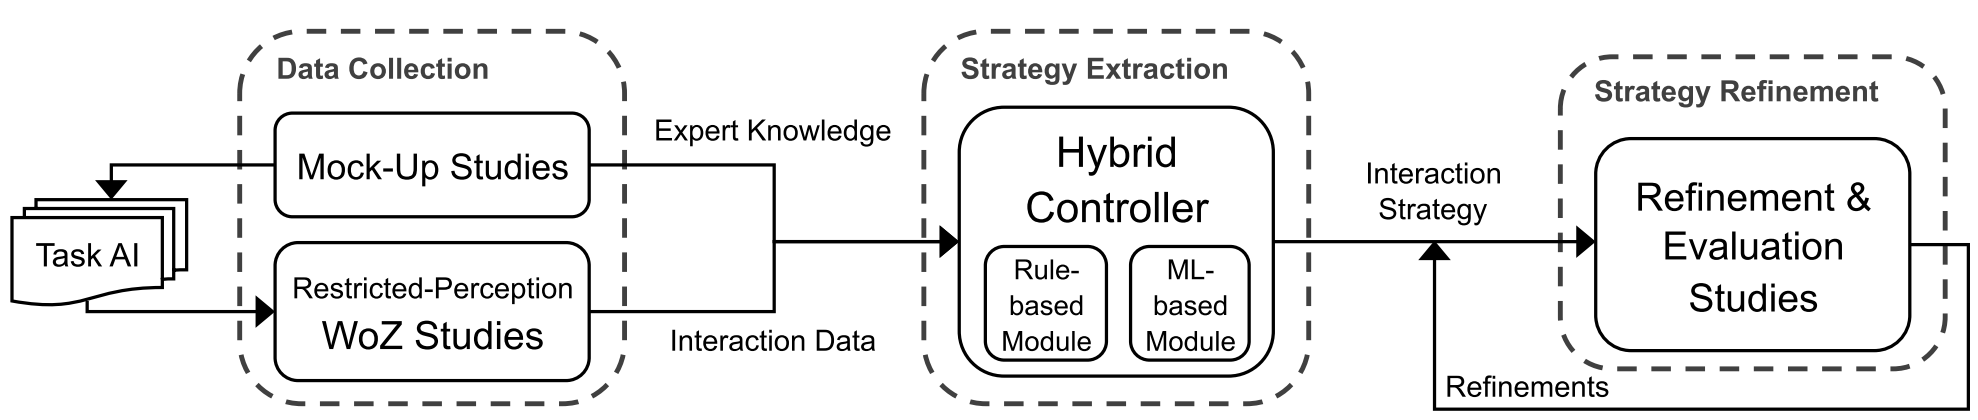
\includegraphics[width=0.85\textwidth]{images/RestrictedPerception_DesignProcess.png}
	\caption{Restricted-perception \ac{WoZ} study methodology. From~\cite{Sequeira2016}.}
	\label{fig:RestrictedPerception_DesignProcess}
\end{figure}




\subsubsection{Virtual Rapport 2.0} \hspace*{\fill} \\
\label{sub:sec:virtualrapport2}

Huang et al., developed a short-term rapport agent to enhance mutual attention and coordination using backchannels through a data-driven approach that takes into account context-specific response models in a dyadic conversational setting~\cite{Buschmeier2011}. The model determines the best suitable timings to generate specific backchannel behaviours and turn-taking opportunities according to the perceptual state observed.

%%%%%%%%%%%%%%%%%%%%%%%%%%%%%%%%%%%%%%%%%%%%%%%%%%%%%%%%%%%%%%%%%%%%%%%%%%%%%%%%%%%%%

\paragraph{\textbf{System description}}

Following Figure~\ref{fig:virtualrapport2System}, the system contains the following modules:
\begin{itemize}
	\item \textbf{\textit{Perception}}: analyses human speaker's behaviour in real time;
	\item \textbf{\textit{Response Models}}: predicts timing of backchannel feedback and end-of-turn opportunities in real time using information from the environment and from the agent itself. It also decides which behaviour to generate;
	\item \textbf{\textit{Generation}}: generates the output from the response models;	
	\item \textbf{\textit{Consensus Data}}: contains data collected from Rapport 06-07 dataset and Self-disclosure data-set (\url{http://rapport.ict.usc.edu}) using \ac{PCS}. The data contains dyadic interactions between a human speaker telling a story and human silent listener.
\end{itemize}

\begin{figure}[hbt]
  \centering
  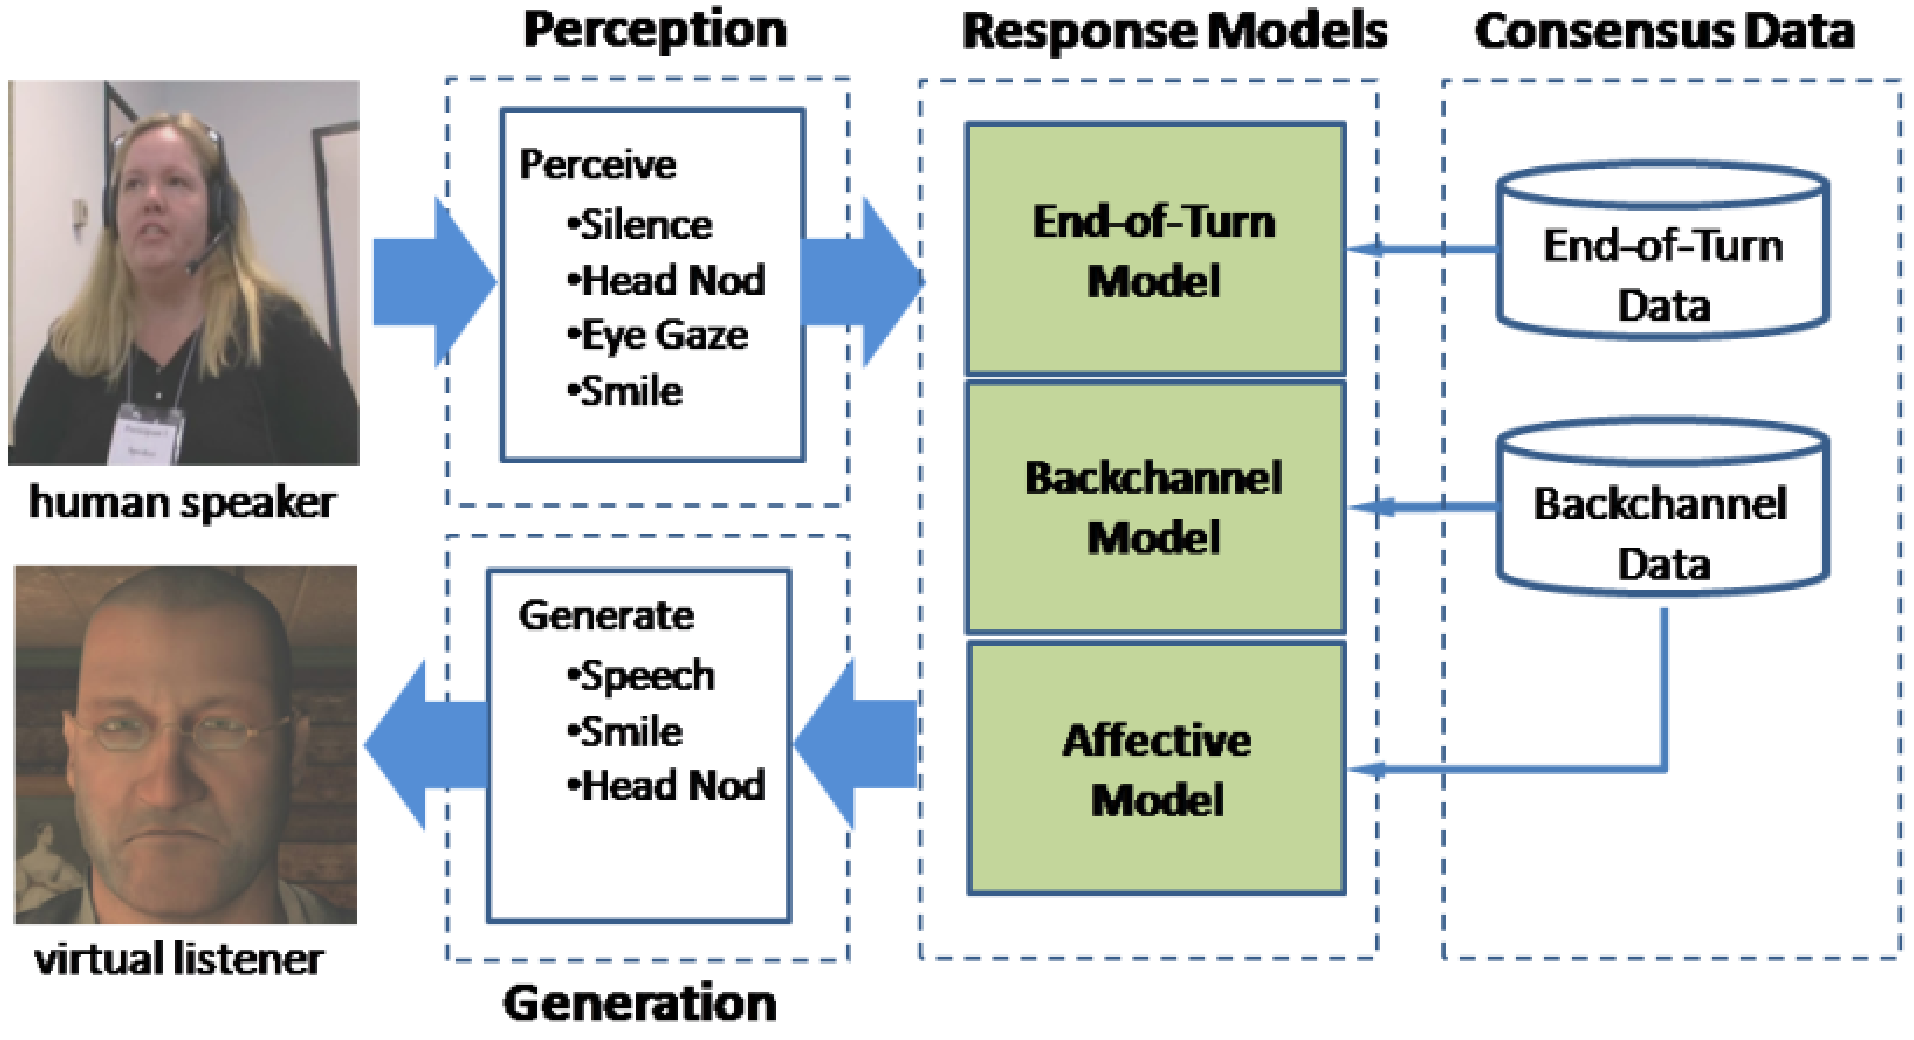
\includegraphics[width=0.8\textwidth]{images/VirtualRapport2_System.png}
  \caption{Architecture of Virtual Rapport 2.0: The \textit{Perception} module analyses human behaviour in real time. \ac{PCS} data is used to create the \textit{Response Models} module. Lastly, the output of the models is generated by the \textit{Generation} module. From~\cite{Buschmeier2011}.}
  \label{fig:virtualrapport2System}
\end{figure} 

As depicted in Figure \ref{fig:virtualrapport2System} there are three models in the \textit{Response Models} module: \textit{End-of-turn}, \textit{Backchannel}, and \textit{Affective}.

The first model, \textit{end-of-turn}, using a rule-based approach, identifies turn-taking opportunities by analysing the current speaker's non-verbal behaviours. For example, if the human interrupts the virtual agent, the agent stops, yields his turn and, says ``I am sorry, keep going'' while showing a facial expression~\cite{Buschmeier2011}.

The second model, \textit{Backchannel}, is \ac{ML}-based (using forward-only inference \ac{CRF} for real-time predictions) and trained using the Rapport 06-07 dataset. It is capable of predicting when and how to give non-verbal feedback.

The last model, \textit{Affective}, analyses facial feature points in real time and detects whenever the speaker is smiling.
 
During the interaction, the three response models are used in conjunction to decide whenever it is appropriate to generate a backchannel. If the speaker is smiling (according to the \textit{Affective} model) and if it is a good opportunity to generate a backchannel (according to the \textit{Backchannel} model) then a head nod (one of the three identified in their studies) is generated accompanied by a smile.

%%%%%%%%%%%%%%%%%%%%%%%%%%%%%%%%%%%%%%%%%%%%%%%%%%%%%%%%%%%%%%%%%%%%%%%%%%%%%%%%%%%%%%%%

\paragraph{\textbf{Evaluation}}
The developed virtual agent interacted with the human subjects in a interview environments in which the former was the interviewer and the later the interviewed. With the goal of comparing the developed system with the previous version~\cite{Gratch2006}, the evaluation measured the following dimensions: rapport (five-item social presence scale~\cite{Bailenson2001}), overall naturalness, backchannel feedback and end-of-turn prediction.


%%%%%%%%%%%%%%%%%%%%%%%%%%%%%%%%%%%%%%%%%%%%%%%%%%%%%%%%%%%%%%%%%%%%%%%%%%%%%%%%%%%%%%%%

\paragraph{\textbf{Discussion}}
The results demonstrates a significant improvement over the previous version. Over 90\% of the users preferred the Virtual Rapport 2.0 rapport agent over the previous rule-based system~\cite{Gratch2006, Morency2008}. The timing's precision and recall are much better, leading to a better synchronism and perceived naturalness from the user during the interaction. According to the authors, the data-driven design, the much richer set of emotions capable of mimicking smiles, and the generation of more natural head gestures might explain the overall better results on the stronger feelings of rapport.

To conclude the most relevant aspects of the system are:
\begin{itemize}
	\item Corpus based approach;
	\item Identification of different head nods patterns;
	\item Duality of \ac{ML}-bases decision and smile to generate backchannel behaviour;
	\item Creative strategy for handling interruptions.
\end{itemize}
\subsubsection{\acl{SAL}} \hspace*{\fill} \\
\label{subsec:AutonomousSensitiveArtificialListeners}

Schröder et al. developed a virtual agent integrated in SEMAINE~\cite{Schroder2010} called \ac{SAL} that has the required capabilities to sustain conversational dialogues and be a good listener~\cite{Schroder2012}.

\paragraph{\textbf{System Description}}

Following the representation of the \ac{SAL} system in Figure~\ref{fig:sensitiveAgent}, the most relevant components are: \textit{Feature extractors}, \textit{Analysers}, \textit{Interpreters}, \textit{Action proposers}, and \textit{Action selection}. The \textit{Feature extractors} component extracts several features such as head gestures, facial features, emotions and, most of all, acoustic features. These features are later analysed by the \textit{Analysers} and \textit{Interpreters} components. The former component analyses non-verbal behaviours and speaker's emotions to produce an estimate of the information's reliability. The later component, given the information available, returns the best state representation for the user, dialogue and agent. Following this, several \textit{Action proposers} will propose an action, in parallel, given previous information. Following, the \textit{Action selection} component selects the action with the highest estimated quality, and lastly, the \textit{Behaviour generator} generates the desired action (utterances and facial animations).

\vspace{-3mm}
\begin{figure}
	\centering
	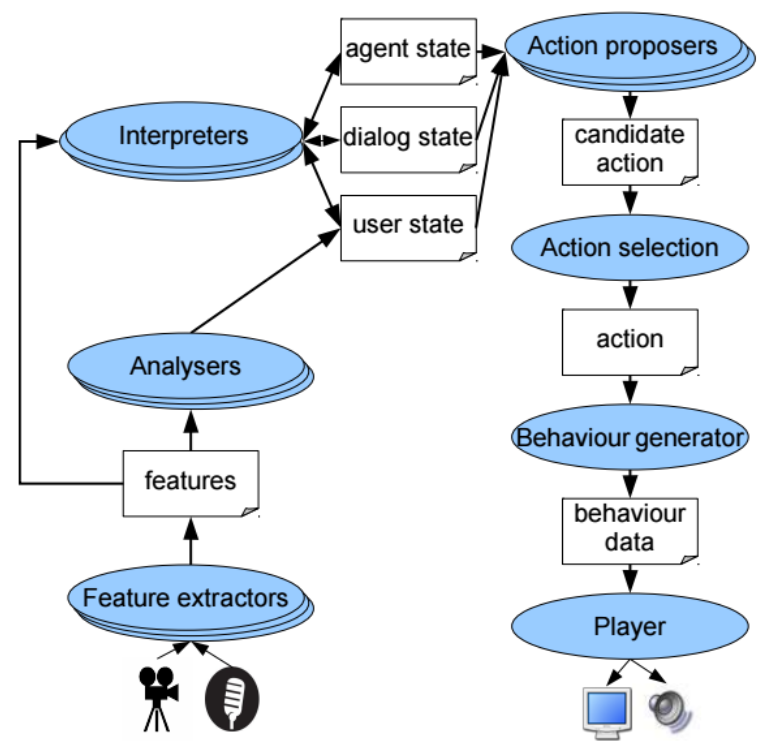
\includegraphics[width=0.5\textwidth]{images/SensitiveAgent.png}
	\caption{\acl{SAL} conceptual architecture. From~\cite{Schroder2012}.}
	\label{fig:sensitiveAgent}
\end{figure}
\vspace{-7mm}

The agent is capable of identifying whether it should be in listener or in speaker mode. This is relevant as the \textit{Action selection} component gives more priority over speaker's actions. An example speaker action would be  saying ``Well?'' or ``Go on, tell me your news!'' after a long pause. In addition, in listener mode, the \textit{Action selection} component chooses the most appropriate backchannel to be produced according to the emotions and interest level estimated from the user.

\paragraph{\textbf{Evaluation}}

The objective was to evaluate if emotion-related abilities influence the quality of human interactions. Firstly the users, with minimal \ac{HRI} experience, receive a introductory briefing on the available personalities they can interact with (4 in total). Then, they can interact twice with each available personality one with the expressive agent, the other with the affective features of the output disabled (randomly). The user interacts with the \ac{SAL} agent's presented in a computer screen (only the face is rendered), using the available cameras and microphones.

\paragraph{\textbf{Discussion}}
There is evidence that expressive abilities may substantially impact the interactions between humans and agents by denoting that flow and perceived engagement was much higher in the emotional \ac{SAL} than in the control environment. Compared with previous described systems, it is one of the most complete models for managing backchannels and turn taking strategies, however, as stated previously in Section~\ref{subsec:Rapport}, attentiveness and coordination are not enough to build rapport, it is also necessary to stimulate positivity which this system does not cover. To conclude, the most relevant aspects of the systems are:

\begin{itemize}
	\item Generate good listeners without understanding semantically what it is being said;
	\item Parallel independent action proposers that uses both rule and \ac{ML} approaches;
	\item Dedicated dialogue management models;
	\item Covers several users affective states by modelling distinct characters.
\end{itemize}
% https://www.lightbluetouchpaper.org/2007/03/14/how-not-to-write-an-abstract/
% http://web.ece.ucdavis.edu/~jowens/biberrors.html

\subsection{Overall Discussion}
\label{subsec:RelWorkDiscussion}

Developing a computational models capable of managing rapport similarly to humans is not an easy feat. Researchers had to focus their research on different aspects of rapport and assess their overall contribution. Table~\ref{fig:comparison:rapportSystems} and Table~\ref{fig:comparison:vh:systems}, respectively, compares the systems regarding how they learn social behaviours, and the used rapport management strategies.

\addtolength{\tabcolsep}{1pt}
\begin{table}
	\centering
	\begin{tabular}{lccccccccccc}
		& \textbf{Type}
		& \textbf{Agent} 
	  	& \rot[70]{\textbf{Gaze}}
	  	& \rot[70]{\textbf{Backchannel}} 
	  	& \rot[70]{\textbf{Small-Talk}} 
	  	& \rot[70]{\textbf{Facial Expressions}}
	  	& \rot[70]{\textbf{Gestures}} 
	  	& \rot[70]{\textbf{Mirroring}} 
	  	& \rot[70]{\textbf{Smile}}
	  	& \rot[70]{\textbf{Turn Taking}}
	  	& \rot[70]{\textbf{Praise}}
	  	\\
	  	\midrule
	  	%%%%%%%%%%%%%%%%%%%%%%%%%%%%%%%%%%%%%%%%%%%%%%%%%%%%%%%%%%%%%%
	  	Mutlu et al.~\cite{Mutlu2006} & Rule-based & Robotic & \cmark & \xmark & \xmark & \xmark & \xmark & \xmark & \xmark & \xmark & \xmark\\
	  	%%%%%%%%%%%%%%%%%%%%%%%%%%%%%%%%%%%%%%%%%%%%%%%%%%%%%%%%%%%%%%
	  	Stanton et al.~\cite{Stanton2014} & Rule-based & Robotic & \cmark & \xmark & \xmark & \xmark & \xmark & \xmark & \xmark & \xmark & \xmark\\
	  	%%%%%%%%%%%%%%%%%%%%%%%%%%%%%%%%%%%%%%%%%%%%%%%%%%%%%%%%%%%%%%
	  	Andrist et al.~\cite{Andrist2015} & Rule-based  & Robotic & \cmark & \xmark & \xmark & \xmark & \cmark & \xmark & \xmark & \xmark & \cmark\\
	  	%%%%%%%%%%%%%%%%%%%%%%%%%%%%%%%%%%%%%%%%%%%%%%%%%%%%%%%%%%%%%%
	  	Mohammad et al.~\cite{Mohammad2010} & \ac{ML}-based  & Robotic & \textbf{?} & \cmark & \xmark & \xmark & \xmark & \xmark & \xmark & \xmark & \xmark \\ 
	  	%%%%%%%%%%%%%%%%%%%%%%%%%%%%%%%%%%%%%%%%%%%%%%%%%%%%%%%%%%%%%%
	  	Huang et al.~\cite{Buschmeier2011} & \ac{ML}-based & Virtual & \xmark & \cmark & \cmark & \cmark & \cmark & \cmark & \cmark & \xmark & \xmark\\
	  	%%%%%%%%%%%%%%%%%%%%%%%%%%%%%%%%%%%%%%%%%%%%%%%%%%%%%%%%%%%%%%
	  	Kok et al.~\cite{Kok2012} & \ac{ML}-based & Virtual &  \xmark & \cmark & \xmark & \xmark & \cmark & \xmark & \xmark & \xmark & \xmark\\
	  	%%%%%%%%%%%%%%%%%%%%%%%%%%%%%%%%%%%%%%%%%%%%%%%%%%%%%%%%%%%%%%
	  	Schröder et al.~\cite{Schroder2012} & \ac{ML}-based & Virtual & \xmark & \cmark & \xmark & \cmark & \cmark & \xmark & \xmark & \cmark & \xmark\\
  		\bottomrule
	\end{tabular}
	\caption{Brief comparison regarding how different virtual agents manage strategies. The systems presented here appear in the same order as in the main body of the text.  \protect\cmark, \protect\xmark \, and \textbf{?}, represents whether the specified strategy is applied, not applied or unclear, respectively.}
	\label{fig:comparison:rapportSystems}
	
\end{table}
\addtolength{\tabcolsep}{-1pt}

Current literature suggests continuing the research on learning social behaviours from \ac{WoZ}~\cite{Sequeira2016, Knox2014, Papangelis2014} studies and use primarily \ac{RL}~\cite{Thomaz2006, Kok2012, Zhao2014, Papangelis2014} classifiers (Section~\ref{subsec:ReinforcementLearning}). This class of algorithms are applicable in rapport as there are sequences of states that will help the agent to know when and how backchannels should be produced in order to build rapport (the reward function). In addition, authors suggest developing solutions capable of adapting current course of actions to the current context of the interaction to improve the quality of virtual agents during interactions~\cite{Kopp2007, Zwiers2011, Reidsma2011, Visser2014}.

\begin{table}[]
	\centering
	\begin{tabular}{|l|c|c|}
		\hline
		\textbf{System}              	& \textbf{Training Source} 	& \textbf{Iterative} \\ \hline
		%%%%%%%%%%%%%%%%%%%%%%%%%%%%%%%%%%%%%%%%%%%%%%%%%%%%%%%%%%%%%%%%%%%%%%%%%%%%%%%%%%%%%%%%%%%%%%%%%
		Mohammad et al.~\cite{Mohammad2010} & Direct Samples (Unsupervised) & Yes \\ \hline
		%%%%%%%%%%%%%%%%%%%%%%%%%%%%%%%%%%%%%%%%%%%%%%%%%%%%%%%%%%%%%%%%%%%%%%%%%%%%%%%%%%%%%%%%%%%%%%%%%
		Virtual Rapport 2.0~\cite{Buschmeier2011} 			& Corpus			& No \\ \hline
		%%%%%%%%%%%%%%%%%%%%%%%%%%%%%%%%%%%%%%%%%%%%%%%%%%%%%%%%%%%%%%%%%%%%%%%%%%%%%%%%%%%%%%%%%%%%%%%%%
		\acf{IPL}~\cite{Kok2012}          				& Corpus \& Subjective evaluation			& Yes \\ \hline
		%%%%%%%%%%%%%%%%%%%%%%%%%%%%%%%%%%%%%%%%%%%%%%%%%%%%%%%%%%%%%%%%%%%%%%%%%%%%%%%%%%%%%%%%%%%%%%%%%
		\acf{SAL}~\cite{Schroder2012} & Corpus \& \ac{WoZ}		& Yes \\ \hline
		%%%%%%%%%%%%%%%%%%%%%%%%%%%%%%%%%%%%%%%%%%%%%%%%%%%%%%%%%%%%%%%%%%%%%%%%%%%%%%%%%%%%%%%%%%%%%%%%%
		Restricted Perception~\ac{WoZ}~\cite{Sequeira2016}  & \ac{WoZ}		& Yes \\ \hline
		
	\end{tabular}
	\caption{Brief comparison of methodologies to learn human social behaviours.}
	\label{fig:comparison:vh:systems}
\end{table}

Most of all, the communication goals of interactions must be considered when developing rapport agents. The context in which the communication partners will interact, the inherent limitations of the virtual agents' perceptions and actions and, most importantly, what kind of emotions and actions we want to elicit from the conversational partner are crucial for the development of such agents. For example, in tutoring applications, mutual gaze plays an important role for increased learning performance \cite{OTTESON1980, SHERWOOD1987, Fry1975}, and in negotiation scenarios not reciprocating negative self-disclosure has ben shown to destroy rapport\cite{Bronstein2012}.




\section{Proposed Solution}
\label{sec:Solution}

The current section describes the proposed solution that will address the development of a robotic rapport agent that improves current models for generating backchannels in dyadic interactions. Following current literature, the solution will inspire on the hybrid system described in Section~\ref{subsec:RestrictedPerceptionsWOZStudy}, on perceptual readings to refine \ac{ML} models described in Section~\ref{subsec:IterativePerceptualLearning}, on the \ac{WoZ} novel approach for training \ac{ML} classifiers described in Section~\ref{subsec:RestrictedPerceptionsWOZStudy}, and, to a lesser degree, current work on iterative systems capable of adjusting their current course of actions in real time~\cite{Kopp2007, Zwiers2011, Reidsma2011, Visser2014} (Section~\ref{sub:sec:ComputationalModelsOfRapport}).

Section~\ref{sub:sec:SERAFramework} briefly describes \ac{SERA} framework that is currently embed on several robotic agents and will support the proposed solution. Section~\ref{sub:sec:solution:arch} describes the rapport agent system architecture and Section~\ref{sub:sec:solution:WoZ} describes the proposed method to train the system in order to produce correct backchannels during the interactions.


\subsection{Supporting Technology}
\label{sub:sec:SERAFramework}

In the research community there are several frameworks to ease the development of virtual agents in \ac{HRI} by promoting reusability between components. Examples of frameworks include SEMAINE~\cite{Schroder2010a}, \acl{VHT}~\cite{Hartholt2013}, \acl{ASAP}~\cite{Kopp2013}, Robot Behaviour Toolkit~\cite{Huang2012}, and \ac{SERA}~\cite{Tullio2015}. The solution will choose the latter as it is being developed internally in \ac{GAIPS}, is used extensively in several \ac{HRI} studies~\cite{Tullio2015}, and was tested in several different embodied robots such as \ac{EMYS} (Figure~\ref{fig:robots:EMYS}) and Keepon (Figure~\ref{fig:robots:Keepon}).

%\vspace{-4mm}
\begin{figure}[ht]
	\begin{minipage}[b]{.4\textwidth}
		\centering
		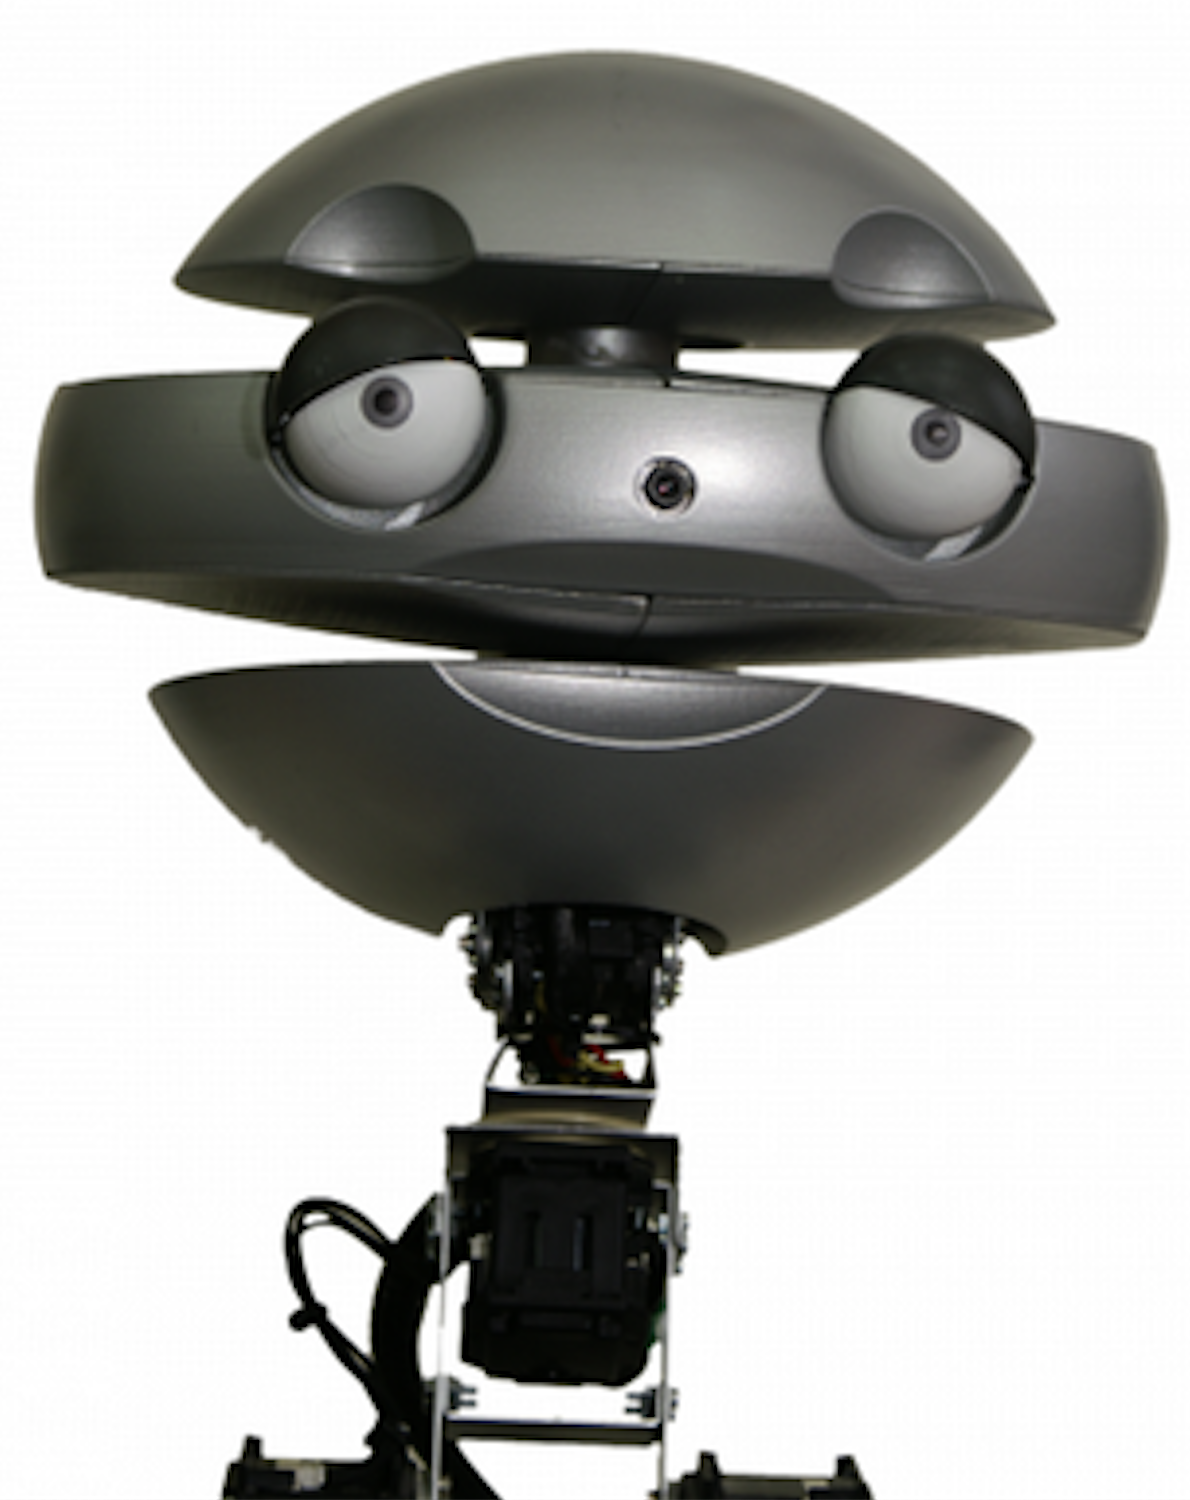
\includegraphics[width=0.4\textwidth]{images/emys.png}
		\caption{EMYS robot.}
		\label{fig:robots:EMYS}
	\end{minipage}
	\hfill
	\begin{minipage}[b]{.4\textwidth}
		\centering
		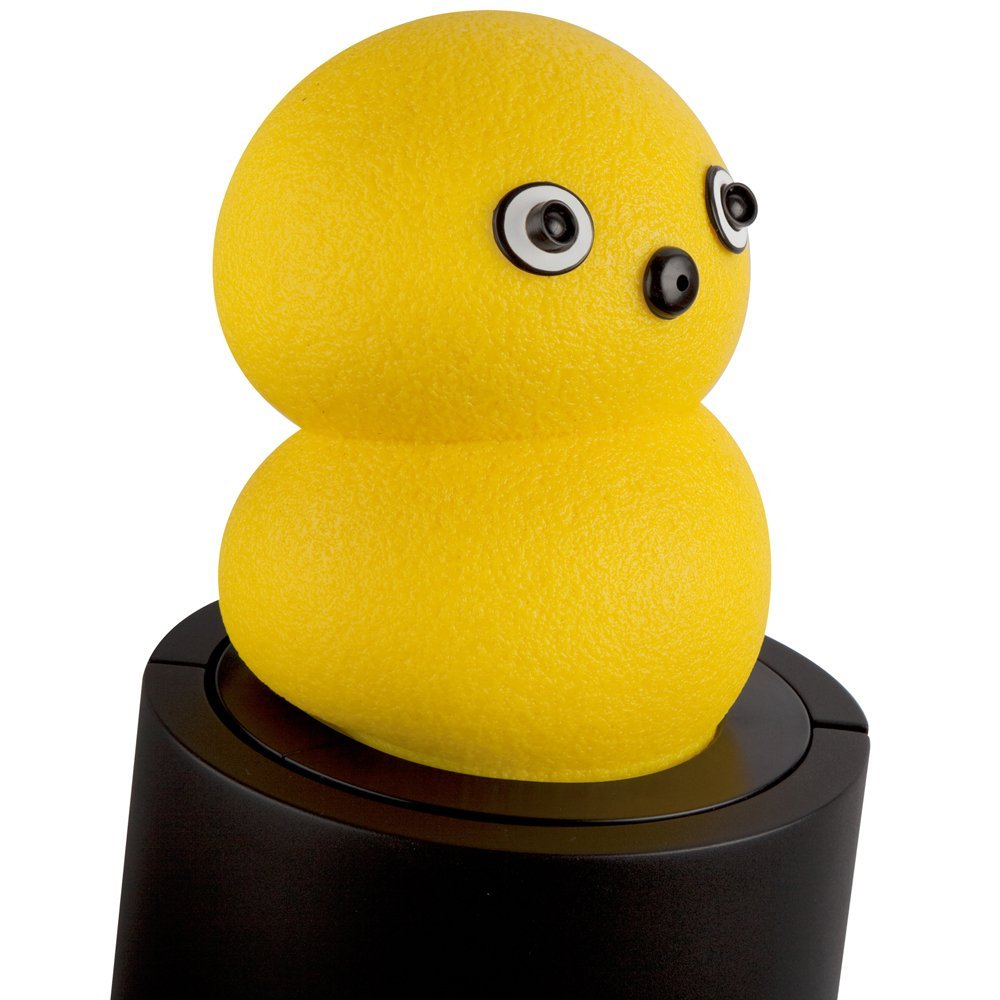
\includegraphics[width=0.4\textwidth]{images/Keepon.jpg}
		\caption{Keepon robot.}
		\label{fig:robots:Keepon}
	\end{minipage}
\end{figure}
%\vspace{-4mm}

\ac{SERA} follows the SAIBA model~\cite{Kopp2006} and is very similar to \ac{ROS}~\cite{Quigley2009} due to, respectively, the separation between intention planning, behaviour planning and realisation, and due to the usage of decoupled modules in an asynchronous messaging system. It aims to be used by both technical and non-technical developers such as psychologists~\cite{Tullio2015}, an advantage as their knowledge is crucial during the development and analysis of \ac{HRI}. For example, utterances are modelled using markup text that can contain non-interrupting behavioural rules and can be developed by non-technical teams.

The most important components are Thalamus, Skene and Nutty Tracks.
\begin{itemize}
	\item \textbf{\textit{Thalamus}}: responsible for receiving and delivering the published messages to the right subscribers;
	\item \textbf{\textit{Skene}}: responsible for translating high-level intentions generated at the decision-making level into a schedule of behaviour actions;
	\item \textbf{\textit{Nutty Tracks}}: responsible for managing animations.
\end{itemize}

\textit{Skene} is the most relevant component in \ac{SERA} for the development of rapport agents as it is the controller that plans animations and non-verbal behaviours such as gaze, utterances and animations according to perceptual messages. This component is rule-based and has an explicit representation of its body position over his physical environment. 

SERA also includes modules for bridging external tools such as \ac{FAtiMA} to model emotions~\cite{Dias2011} or Unity to create virtual scenarios. All these modules co-exist inside the \textit{Thalamus} ``network'' to cooperate, in order to achieve the interactional goals in any \ac{HRI} scenario (e.g., negotiation scenarios on Figure~\ref{fig:SERA:Examples}).

\begin{figure}
	\centering
	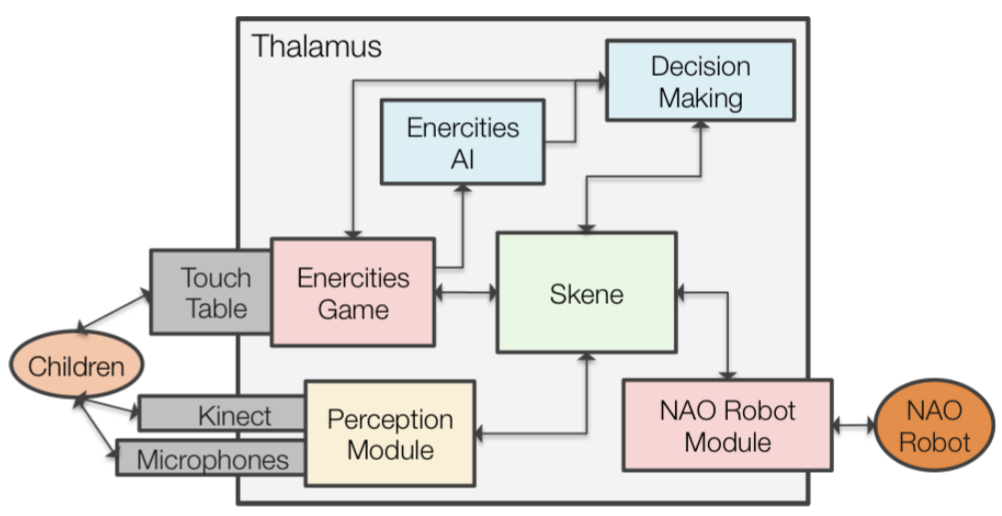
\includegraphics[width=0.6\linewidth]{images/SERA_ExSystemEC.png}
	\caption{Enercities scenario system architecture integrated with SERA framework. From~\cite{Tullio2015}.}
	\label{fig:SERA:Examples}
\end{figure}
%\vspace{-4mm}

Despite being under development, \ac{SERA} is stable and demonstrates its applicability in a wide range of \ac{HRI} scenarios. However, the \textit{Skene} component lacks rapport management strategies and it does not adapt its actions when interrupted by the user, which reduces coordination and the overall feeling of rapport. Moreover, the \textit{Skene} component is rule-based which is not sufficiently elegant to build systems more appealing and natural to end-users.
\subsection{Architecture}
\label{sub:sec:solution:arch}

In order to evaluate the proposed backchannel behaviour generation \ac{ML} classifier we require a robotic rapport agent to be tested on human subjects. We propose extending \ac{SERA} framework to manage rapport by providing tools for stimulating positivity, coordination, and mutual attention (similar to Figure~\ref{table:BuildingRapportPlan} on Section~\ref{subsec:Rapport}) enabling flexibility, and reusability in different scenarios. Despite backchannel behaviours being more targeted to enhance mutual attention and coordination, we intend to stimulate positivity as well, by using specific interactional rules.

The architecture that will instantiate the above proposal is depicted in Figure~\ref{fig:rapport:archicture}. The system decision making process is managed by the \textit{Rapport Controller} Module that contains three components: a rule-based and two \ac{ML}-based components.

\begin{figure}
	\centering
	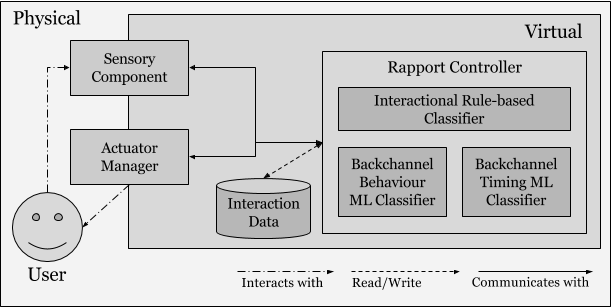
\includegraphics[width=0.75\textwidth]{images/Rapport_archtu.png}
	\caption{Partially decided Rapport Architecture proposal.}
	\label{fig:rapport:archicture}
\end{figure}

The rule-based component is responsible for managing high-level interactional rules that are easier to specify, for example, compliment cooperation actions to stimulate positivity. These rules can be either context specific, or generic enough to be included in other scenarios. The \textit{Interactional Data} data storage depicted in Figure~\ref{fig:rapport:archicture} containts relevant information to manage the interaction.

Two \ac{ML}-based components will handle more complex perceptual states that may arise during the sessions and that would be hard to explicitly define behavioural rules. One module will return correct timings for the generation of backchannels and the other will return the most fitting backchannel behaviour. For example, the first module will suggest that the current instance is appropriate, and the second module will return head nod as the most adequate social behaviour. The retrieved features should be as context independent as possible, including features such as facial expression, head nod frequency, presence of a smile, silence duration, and gaze position. The dominant \ac{ML} classifier is \acf{RL} (Section~\ref{subsec:ReinforcementLearning}) as it was suggested by several authors~\cite{Thomaz2006, Kok2012, Zhao2014, Papangelis2014}.

The \textit{Rapport Controller} will redirect perceptual information collected from the \textit{Sensory Component} and \textit{Actuator Manager} to its component, and will analyse the returned result. From it, the controller will decide which actions should be initiated, maintained or even interrupted. With the bidirectional relationship between the \textit{Rapport Controller}, the \textit{Sensory Component}, and the \textit{Actuator Manager}, we aim to extend \ac{SERA} to support interruptible actions and allow quick adjustments to the agent's behaviour and build better rapport~\cite{Reidsma2011, Visser2014, Kopp2007, Zwiers2011}. For example, similarly to the agent described in Section~\ref{sub:sec:virtualrapport2}, interrupting current speech acts whenever the user starts to speak.

Conflicts may arise between the rule-based component and the \ac{ML}-based components. If the generated behaviours do not conflict with each other, e.g. gaze target and smiling, both actions are executed by the agent. If the generated behaviour conflicts with another, then the \ac{ML}-based components take priority over the rule-based. If there is conflict between two rules, the one with the highest priority takes place (e.g., silence over vocalisation when detecting user's speech).
\subsection{Learning Subconscious Behaviours}
\label{sub:sec:solution:WoZ}

Both \ac{ML}-based modules proposed in Section~\ref{sub:sec:solution:arch} need to be trained in order to learn how to generate correct backchannels. Note, as mention in Section~\ref{subsec:RestrictedPerceptionsWOZStudy}, that in \ac{WoZ} the human subject is not aware that the agent is being controlled manually (partially or fully) by another human, the wizard. In the traditional \ac{WoZ}, the wizards have full access to what is happening in the scenario and have control over the virtual agent, using a \ac{UI}. However, as aforementioned by Sequeira et al., it is relevant to take into account that the virtual agent has inherent limitations in their perceptional abilities and their actions onto their external world~\cite{Sequeira2016}. Moreover, social behaviours are mostly done subconsciously, therefore, the experiment could be influencing the results by just forcing the user to rationalise over what is being subconsciously felt. Taking this two issues into account, we propose an approach for learning correct backchannel generation in virtual agents and embodied agents in \ac{HRI} using limited-perception \ac{WoZ} and human experts for corrective feedback (Figure~\ref{fig:learning:process}).



\begin{figure}
	\centering
	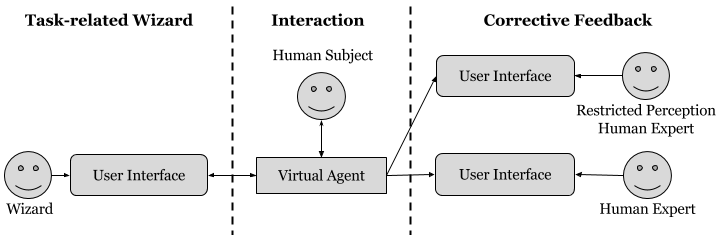
\includegraphics[width=\textwidth]{images/CorrectiveFeedbackRestrictiveWoZ_Diagram.png}
	\caption{Using perceptual readings and limited perception \ac{WoZ} to assess backchannels quality. Human experts monitor the interaction and provide corrective feedback according to their perceptions. The task-related wizard is optional.}
	\label{fig:learning:process}
\end{figure}

Following Figure~\ref{fig:learning:process}, one wizard is responsible for controlling the virtual agents task-related actions and two human experts for providing corrective feedback regarding whether the agent's behaviour is socially appropriate or inappropriate~\cite{Kok2012, Poppe2011}, using a \ac{UI}. One human expert will have its perceptions limited with same extent as the virtual agent, and the other will have unrestricted perceptions. This approach can be seen as reverse-\ac{RL} since it is possible to map the human experts feedback to a reward function, in which, appropriate and inappropriate backchannels will have values values $1$ and $-1$, respectively.

Using this approach it is possible to obtain multiple feedback over the generated behaviours, similar to \ac{PCS}~\cite{Huang2010} without influencing the results by forcing the users to rationalise their actions. Cohen's kappa coefficient $\kappa$ may be used to measure inter-rated agreement between two human experts (Equation~\ref{eq:CohenKappa}). In the equation, $p_0$ is the relative observed agreement and $p_e$ the probability of random agreement.


\vspace{-3mm}
\begin{equation}
	\label{eq:CohenKappa}
	\kappa = \frac{p_0 - p_e}{1 - p_e}
\end{equation}

With the data collected using the restricted-perception \ac{WoZ}, the data will be pre-processed and used to train the \ac{ML}-based component using Weka~\cite{Hall2009}. \ac{RL} algorithms will take priority since they were the main suggestion from several authors~\cite{Thomaz2006, Kok2012, Zhao2014, Papangelis2014, Blumberg2002, Andrist2015, Mutlu2006}. Nevertheless, similar approaches can be further investigated. 

As summarised in equation~\ref{eq:IterativeSolutionEquation}, the system evolves as follows. The initial version $M_0$ is the only version that is strictly rule-based and stripped of previous knowledge according to the information collected from preliminary studies, and the interactional goals. The goal of $M_0$ is to explore as many state combinations as possible in order to produce great number of backchannels, and acquire, as much corrective feedback as possible from the human experts~\cite{Kok2012}. The corrective feedback collected on $M_n$ is later used to train $M_{n+1}$ version of the rapport agent. Following this pattern, we expect $M_n$ to build better rapport than the previous $M_{n-1}$ version. Note that, after the first learning state, the initial excessive backchannels rules must be discarded and replaced by the \ac{ML} generated backchannels, similar to how \ac{IPL} (Section~\ref{subsec:IterativePerceptualLearning}) discards the negative samples after the first subjective evaluations. 

\vspace{-3mm}
\begin{equation}
	\label{eq:IterativeSolutionEquation}
	M_{n+1} = M_{n} + Corrective\, Feedback
\end{equation}

To conclude, after several iterations~\cite{Sequeira2016, Kok2012}, the best possible model $M_n$ will be one tested on users, in which human experts are not required to be present since the agent does not benefit from further training. The final system should represent the average listener's behaviour interacting with the average speaker. Preliminary studies may be conducted to assess the feasibility of the proposed learning strategy.
\section{Evaluation}
\label{sec:Evaluation}
The current section will describe the methodology that will be used in order to evaluate the correctness and benefits of the proposed solution. 

The proposed solution aims to improve current backchannels models and test the developed model on a robotic rapport agent. Robot \ac{EMYS} will be used due to its expressiveness, and the negotiation scenario will be simplified version of Split Or Steal~\cite{VandenAssem2012}, due to its simplicity and because it was previously integrated in the \ac{SERA} framework. Split Or Steal requires two players that will discuss how a large amount of money will be shared among the players. After a brief initial discussion, each player will have to choose one of two spheres that will decide the outcome of the game: \textit{Split} or \textit{Steal} (Table~\ref{fig:splitOrSteal}).

\begin{table}[]
	\centering
	\begin{tabular}{|l|c|c|}
		\hline
		\textbf{Player1/Player2} & 
		\textbf{\textit{Steal}} & \textbf{\textit{Split}} \\ \hline
		\textbf{\textit{Steal}} & $0,0$ & $2,0$		\\ \hline
		\textbf{\textit{Split}} & $0,2$ & $1,1$      \\ \hline
	\end{tabular}
	\caption{Split Or Steal payoff matrix. Both players lose the money if they both decide to \textit{Steal} and the money is divided in half if both players decide to \textit{Split}. The remaining options leads to the \textit{Steal} player keeping all the money.}
	\label{fig:splitOrSteal}
\end{table}

\vspace{-8mm}

The evaluation of the proposed solution must into three main issues:
\begin{itemize}
	\item Correctiveness of the generation of backchannel behaviour;
	\item User preference of the trained system over the untrained version (rule-based);
	\item Assess the impact of rapport in cooperation in negotiation scenarios.
\end{itemize}

We will investigate previous literature to assess what are the most important features and interactional rules in these types of games. With this knowledge we will define what are the set of actions and perceptual capabilities that \ac{EMYS} should have to be successful in building rapport, and define the initial version of the system, $M_0$, solely rule-based and and stripped of previous knowledge. The baseline for evaluation will be a lighter version of $M_0$ that tries to balance when and how to generate backchannels without the eagerness to generate more backchannels in order to have more corrective feedback.

The evaluation process will focus on studying how version $M_n$ represents an improvement over previous version $M_{n-1}$. Human subjects (at least 30 from the university to ensure statistical viability) will interact with the version $M_n$ of the rapport agent (with $n={1,2,...,n}$) while human experts (from the research group) provide corrective feedback. After each session, each person will answer a questionnaire in order to evaluate their individual experience. This questionnaire aims to measure the users perception of rapport on the embodied agent using:

\begin{itemize}
	\item Adapted version of \acf{IRI}~\cite{Davis1980};
	\item Godspeed series~\cite{Bartneck2009};
	\item Five-item social presence scale~\cite{Bailenson2001};
	\item Engagement using task specific questionnaire.
\end{itemize}

The inter-rated agreement between the human experts will be measured using Cohen’s kappa coefficient (Equation~\ref{eq:CohenKappa}) and the the trained models will be objectively measured for precision (Equation~\ref{eqn:precision}) and recall (Equation~\ref{eqn:Recall}). The initial \ac{RL} values (Equation~\ref{eq:QLearning}): learning rate $\alpha$, discount value $\gamma$, and the initial reward function $R(s_t,a_t,s_{t+1})$ will be studied to verify which combination leads to better results (Section~\ref{subsec:ReinforcementLearning}).

Lastly, we expect the last version of the system, $M_n$ to be able to build rapport, provide better backchannel feedback and elicit more cooperation from the users in the negotiation scenario.

%%%%%%%%%%%%%%%%%%%%%%%%%%%%%%%%%
%%%%%% RAW
%%%%%%%%%%%%%%%%%%%%%%%%%%%%%%%%%

%According to previous studies [33 dont stare at me], during dyadic interactions, the listener usually maintains long gazes at the speaker and only interrupts briefly from time to time. 

%In fact, [9 toward dyadic...] found that in a negotiation setting not reciprocating negative self-disclosure led to decreased feelings of rapport.  \cite{Bronstein2012} 

%mutual gaze in determine turn-taking turn-taking [8] [12] [14] [56] [47] [vêm do dont stare at me]. 

%One of the most notable non-verbal behaviors to build rapport is gaze because it is a clear signal of mutual attention, acts as an invitation to interaction, increases dynamism, likelability and believability [4 do dont stare at me]



%%%%%%%%%%%%%%%%%%%%%%%%%%%
%%5 dont stare at me %%%%%%
%its impact in a wide range of interpersonal domains includ- ing social engagement [52], classroom learning [22], suc- cess in negotiations [20], improving worker compliance [18], psychotherapeutic effectiveness [59], and improved quality of child care [11].

%Gaze as object of interest [8] [37] [55]. , effects on the way communication proceeds [54] [60] [23] [19] [28].

%\item Head gestures; %[7 do virtual rapport 2.0] refere q aumenta persuacao

%%%%%%%%%%%%%%%%%%%%%%%%%%
%%%%%%%%%%%%%%%%%%%%%%%%%%


%%%%%%%%%%%%%%%%%%%%%%%%%%
% POTENTIAL RAPPORT RULES
%%%%%%%%%%%%%%%%%%%
% dint stare at me
%In fact, previous work demonstrated that there is evidence that in health domains, high rapport doctors engaged in less extensive eye-contact than low rapport doctors  , 85\% and 70\% of the interaction time respectively . However, the impact of the gaze depends if the interacts are in a helping context (e.g. meetings with a doctor) or in a non-helping context (e.g. interviewing)  [dont stare at me].  On the latter, directed gaze is correlated positively with participant’s evaluative impression [ Tickle-Degnan and Rosenthal]. In interviweing ocntexts, Goldberg, Kiesler, and Collins [25] found that people who spent more time gazing at an interviewer received higher socio- emotional evaluations. 

%Argyle [1] found that in dyadic conversa- tions, the listener spent an average of about 75% of the time gazing at the speaker.

%Kendon [33] reported that a typical pattern of interaction when two people converse with each other consists of the listener maintaining fairly long gazes at the speaker, interrupted only by short glances away.

%In short, gaze can also have negative impact if not dosed correctly.
%%%%%%%%%%%%%%%%%%%%%%%%%%
\section{Conclusion}
\label{sec:Conclusion}

The state-of-art in rapport agents suggests that it is very difficult to implement a computational model capable of managing rapport similarly to humans. However, by restricting such models, it is possible to create imperfect systems that are capable, at some length, to increase rapport between agents and humans. There are not many agents with data-driven components for managing rapport in \acl{HRI}. Most of the \ac{ML}-based current agents use data-driven classifiers to improve their task performance and not, as we intend, improve their social behaviour performance.

The current state-of-the-art covers two classes of systems. On one hand, rule-based systems are easier to develop but are more rigid, on the another, \ac{ML}-based systems are more effective on generating behaviours that are perceived as more natural by humans. Moreover, some authors have been working on continuous interaction systems that are capable of interrupting or even adapting their current set of active actions. Other researchers have been working on agents that pro-actively seek task-related information to complement their knowledge and improve their results.

The proposed solution aims to create a robotic rapport agent that takes the best of both rule-based and \ac{ML}-based systems, and a novel approach for learning backchannels using restricted-perception \ac{WoZ} and human experts for corrective feedback. Following the tendency and suggestions made by researchers, we will use \ac{RL} as the dominant classifier (albeit other classifiers may be considered) and we will repeat the learning stage until there are signs of convergence. The developed solution will be internally incorporated in \ac{SERA} framework that is being actively developed in \ac{GAIPS}, has been used extensively to conduct several studies and it is well integrated with \ac{EMYS}.

To assess the performance, the untrained system (rule-based) will be compared with the trained system in a negotiation scenario, Split Or Steal using robot \ac{EMYS}. We expect the backchannel model, and therefore the rapport agent, after some iterations, to be able to produce more natural backchannels than the untrained system, and elicit more cooperation from the adversary by building rapport.

The development of the proposed work will follow the schedule presented in Appendix~\ref{app:Planning}.
%\section*{Acknowledgment}
The author would like to thank...

\newpage

%%%%%%%%%%%%%%%%%%%%%%%%%%%%%%%%%%%%%%%%%%%%%%%%%
% References
\bibliographystyle{splncs}
\bibliography{bib/IEEEabrv, bib/Bibliografia, bib/BibliografiaOther}
%%%%%%%%%%%%%%%%%%%%%%%%%%%%%%%%%%%%%%%%%%%%%%%%%

% This is the ACRONYMS Definition
\begin{acronym}[H.264/SVC]
	\acro{API}{Application Program Interface}
	\acro{HD}{High Definition}
	\acro{HDTV}{High Definition Television}
	\acro{IP}{Internet Protocol}
	\acro{IT}{Information Technology}
	\acro{LAN}{Local Area Network}
	\acro{OS}{Operating System}
	\acro{P2P}{Peer-to-Peer}
	\acro{TCP}{Transport Control Protocol}
	\acro{UDP}{User Datagram Protocol}
	\acro{UI}{User Interface}
	\acro{URL}{Uniform Resource Locator}
	\acro{WLAN}{Wireless Local Area Network}
	\acro{XML}{Extensible Markup Language}
	\acro{IST}{Instituto Superior Técnico}
	\acro{NLP}{Natural Language Processing}
	\acro{POS}{Part-of-speech}
	\acro{SVM}{Support Vector Machine}
	\acro{ME}{Maximum Entropy}
	\acro{ML}{Machine Learning}
	\acro{GAIPS}{Intelligent Agents and Synthetic Characters Group}
	\acro{IPL}{Iterative Perceptual Learning}
	\acro{PCS}{Parasocial Consensus Sampling}
	\acro{SVM}{Suport Vector Machine}
	\acro{HRI}{Human-Robot Interaction}	
	\acro{NLP}{Natural Language Processing}	
	\acro{WoZ}{Wizard-of-Oz}
	\acro{IRI}{Interpersonal Reactivity Index}
	\acro{CRF}{Conditional Random Field}
	\acro{SERA}{Socially Expressive Robotics Architecture}
	\acro{AI}{Artificial Intelligent}
	\acro{ROS}{Robot Operating System}
	\acro{RL}{Reinforcement Learning}
	\acro{EMYS}{EMotive headY System}
	\acro{IRI}{Interpersonal Reactivity Index}
	\acro{VHT}{Virtual Human Toolkit}
	\acro{ASAP}{Artificial Social Agent Platform}
	\acro{FAtiMA}{Fearnot AffecTIve Mind Architecture}
	\acro{BML}{Behaviour Markup Language}
	\acro{MDP}{Markov Decision Processes}
	\acro{SAL}{Sensitive Artificial Listeners}
	\acro{FML}{Function Markup Language}
	\acro{GUI}{Graphical User Interface}
	\acro{SSI}{Social Signal Interpretation}
	\acro{AU}{Action Unit}
	\acro{WPF}{Windows Presentation Foundation}
	\acro{TTS}{Text-To-Speech}
\end{acronym}

%%%%%%%%%%%%%%%%%%%%%%%%%%%%%%%%%%%%%%%%%%%%%%%%%
% Appendices
\newpage
\appendix

\begin{landscape}
	\section*{Appendices}
	\section{Planning}
	\label{app:Planning}
	
	\begin{figure}	
		\centering 
		\adjincludegraphics[angle=0,width=1.55\textwidth, trim={{.04\width} {.5\height} {.04\width} {.05\height}},clip]{partial/Planeamento.pdf}
	\end{figure}
	
\end{landscape}
%%%%%%%%%%%%%%%%%%%%%%%%%%%%%%%%%%%%%%%%%%%%%%%%%

\end{document}